\documentclass[../main.tex]{subfiles}


\begin{document}

When identifying the approach and metrics, we divided our research into three primary categories: architecture, device handshake, and system monitoring and security. Architecture encompasses the physical hardware architecture, how devices are connected together, how edge device traffic is routed and structure. Device handshake analyzes ways of creating trust between edge devices and gateways. System monitoring and security focuses on security between devices and gateways, as well as, active monitoring devices and gateways in an effort to maintain a healthy system. 


\section{Approach}

The approach overview describes how we will investigate each area of focus we defined. 

\subsection{Architecture}
Internet of Things architecture can be divided into three primary layers: application layer, transport layer, and sensing layer. The sensing layer is the bottom layer. In the sensing layer, edge devices including sensors and actuators, will report their environment to the transport layer or perform specified task provided by the transport layer. 

The middle layer is the transport layer. The transport layer includes gateways and networking protocols that are responsible for transferring data between the sensing layer and the application layer. Current architectures include a single tier of gateway devices within the transport layer, which is displayed in figure~\ref{fig:sing_tier}. 
The application layer, the top layer, includes cloud services where data can be stored, user applications, and data mining services. 

\begin{figure}[!htb]
    \centering
    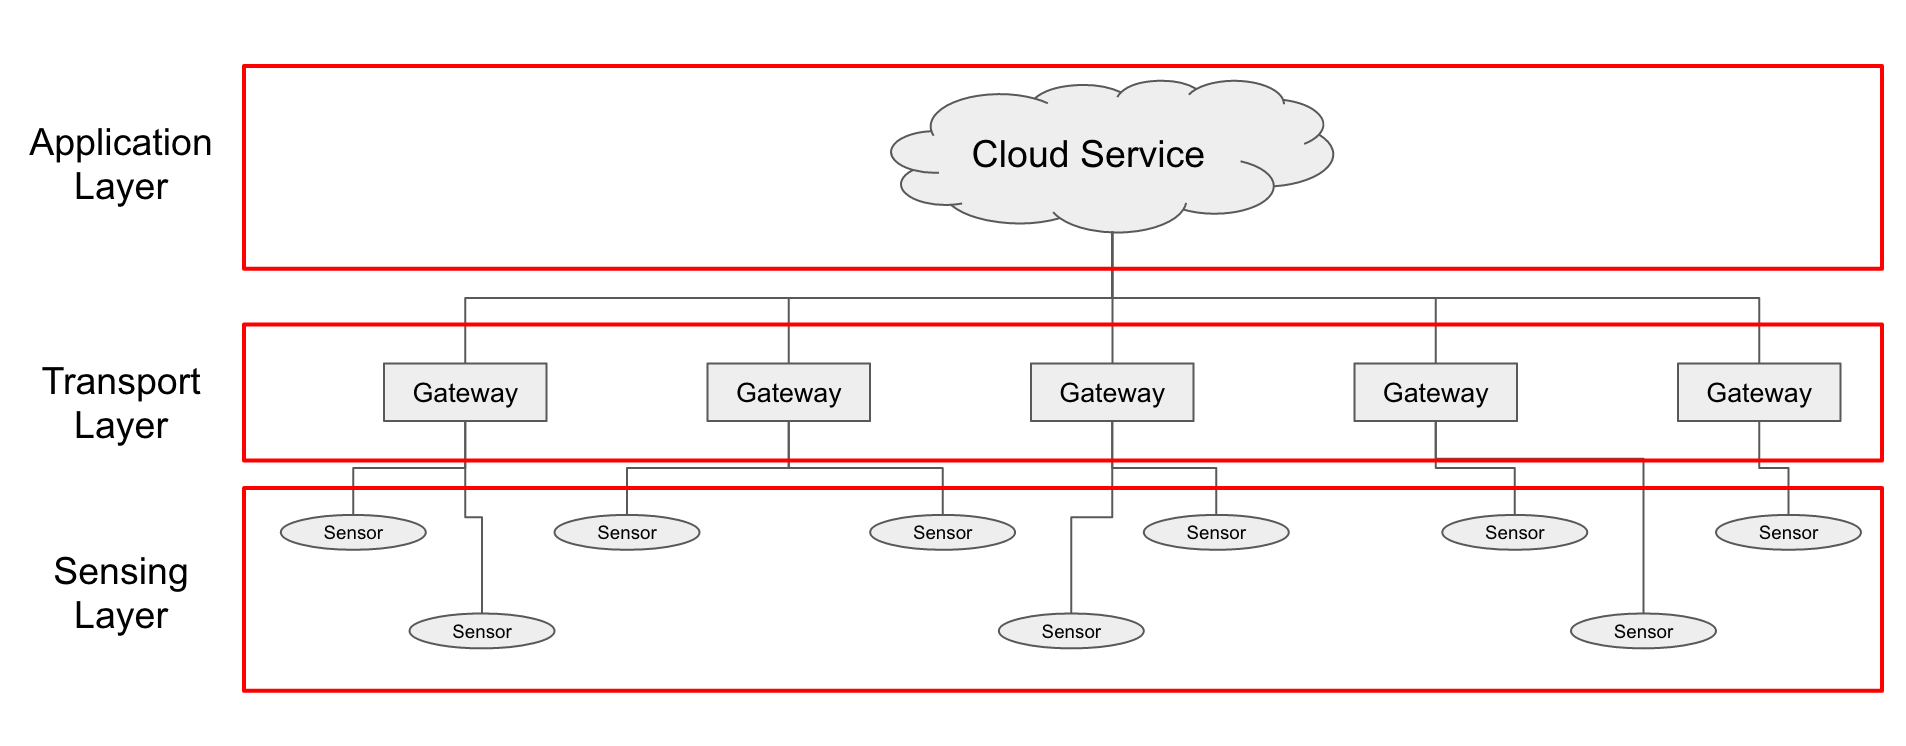
\includegraphics[scale=.35]{single-tier.png}
    \caption{Single-tiered Architecture}
    \label{fig:sing_tier}
\end{figure}

We propose the expansion of a fog architecture to CPS by adding decision-making within the transport layer and multiple tiers of gateways. The decision layer would contain machine learning and other predictive techniques to determine the health of the subsystem within the sensing and transport layers. Multiple tiers of gateways would provide redundancy within the transport layer to help reduce single failure points. Figure~\ref{fig:multi_tier} displays the multi-tier gateway approach. As the system scales up, a coalition of gateways will be used to determine the most effective manner of routing edge device traffic. We will investigate systems of size 10, 100, 1000, and 10000 to understand how systems change as the number of devices increase. We will investigate the optimal number of gateways as the system scales, as well as, the optimal number of tiers for these gateways. 

We will begin by creating single-tiered and multi-tiered CPS and monitor normal health by collecting sensor data, transmission speed, number of transmissions, and number of active sensors in the system. After the baseline data has been created, single failure points, intrusion, and other malfunctions/attacks will be introduced to the system to test effectiveness of both architectures. For each test, we will calculate the number of active sensors, the time to return to a functioning state, and the resources used to return to a functional state.



\subsection{Routing Protocol}
For routing, we will begin by investigating mobile ad-hoc network (MANET) \nomenclature{MANET}{Mobile Ad-hoc Network} routing protocols including Optimized Link State Routing Protocol (OLSR) \nomenclature{OLSR}{Optimized Link State Routing Protocol}, Destination Sequenced Distance Vector Routing Protocl (DSDV) \nomenclature{DSDV}{Destination Sequenced Distance Vector Routing Protocol}, and Ad-hoc On Demand Distance Vector Protocol (AODV) \nomenclature{AODV}{Ad-hoc On Demand Distance Vector Protocol}. OLSR and DSDV are proactive routing protocols that maintain a routing table that is periodically updated through control message \cite{7724222,7724851}. AODV is a reactive routing protocol that uses Bellman-Ford Distance Vector Routing Algorithm to determine the shortest connection between the devices \cite{7724222}. These protocols provide a method for routing traffic, however, they do not take into account the current load on the gateway or secondary connections for the edge devices. We will investigate adapting these algorithms for our routing protocol. 

%\begin{figure}
%    \centering
%    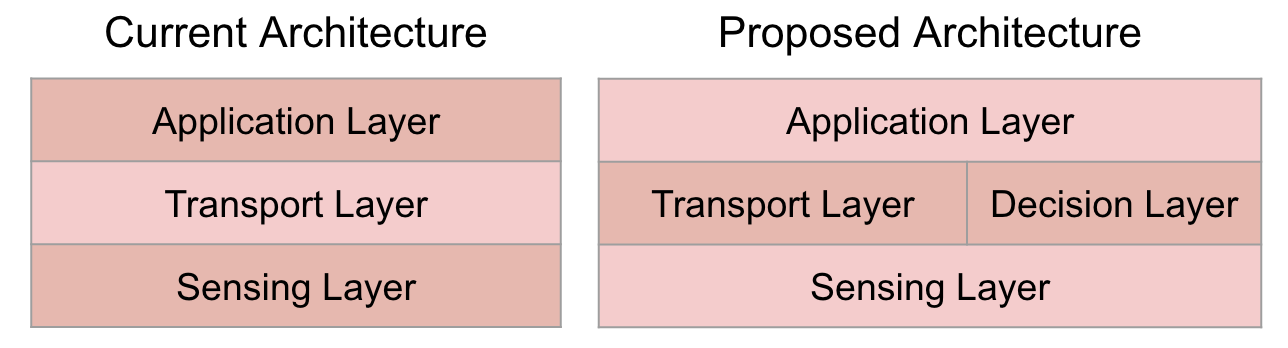
\includegraphics[scale=.35]{arch.png}
%    \caption{Architecture Approaches}
%    \label{fig:arch_approach}
%\end{figure}



\begin{figure}[!htb]
    \centering
    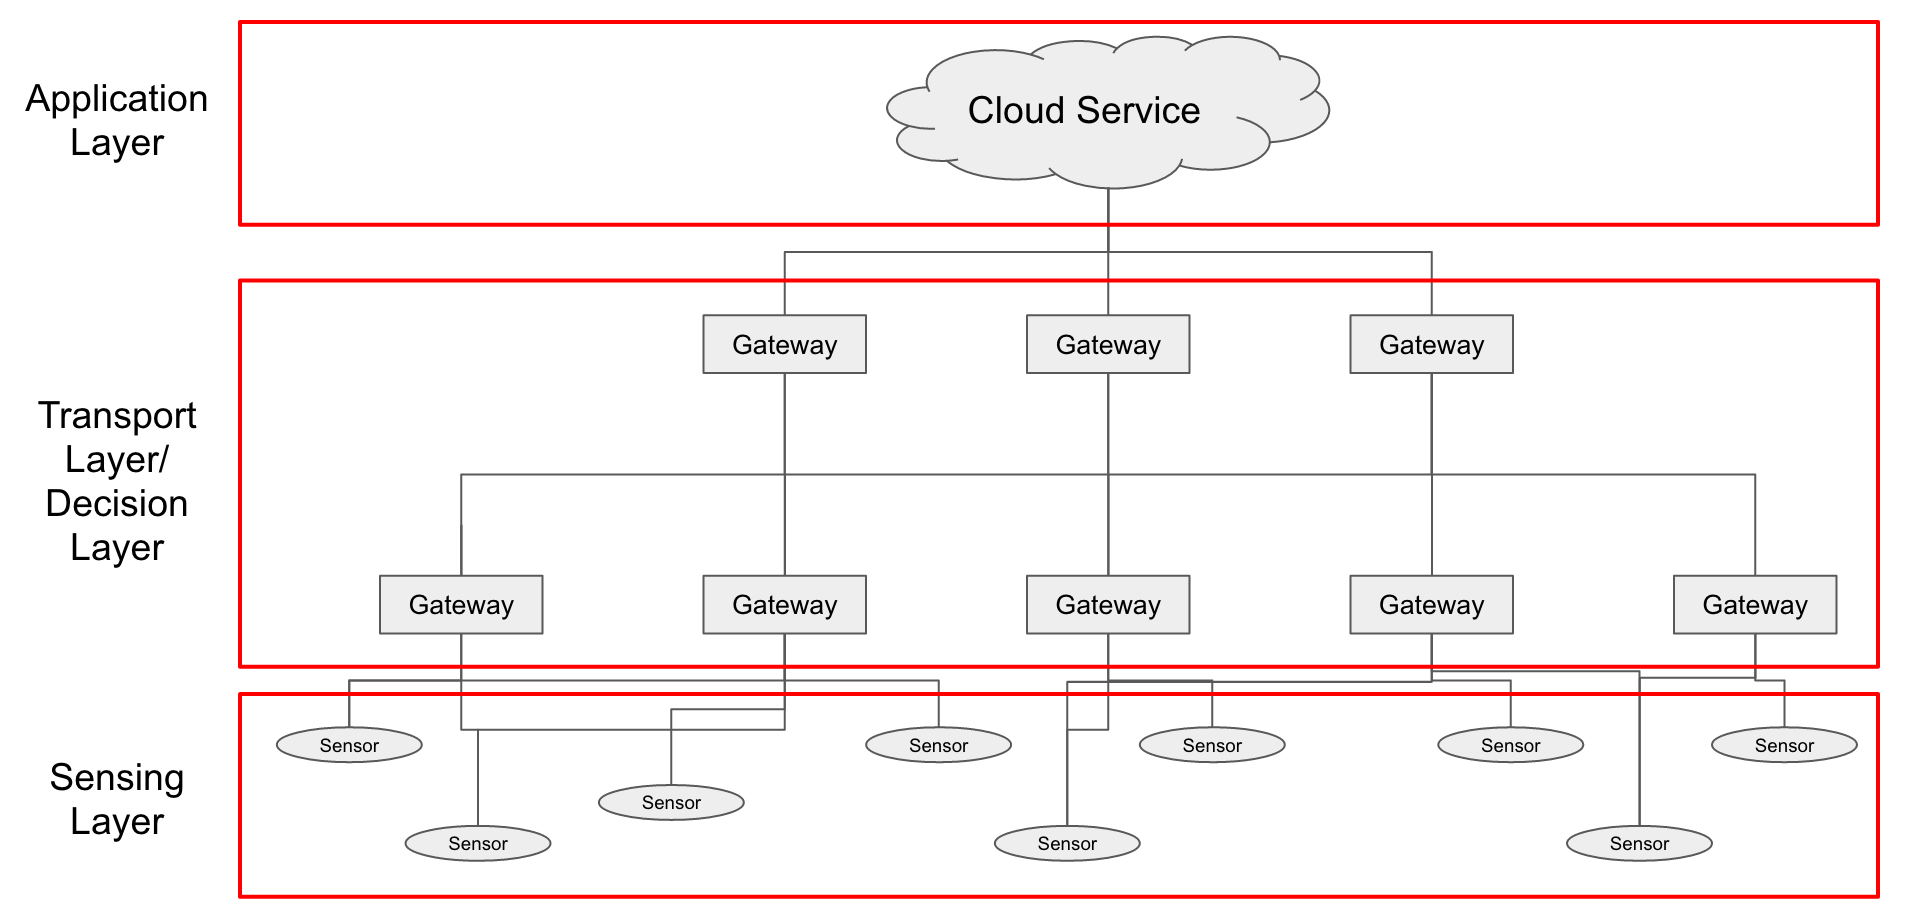
\includegraphics[scale=.35]{multi-tier.png}
    \caption{Multi-tiered Architecture}
    \label{fig:multi_tier}
\end{figure}

% Is this done elsewhere?

\subsection{Device Handshake}

Devices within an IoT architecture need a secure, quick, and efficient way to connect with each other. To provide this level of authentication, we will test multiple methods of device handshakes in an effort to determine the effectiveness of each handshake. We will investigate the use of certificate authentication between end devices and gateways and multiple encryption techniques and keys to authenticate the devices. To begin, we will analyze AWS IoT X.509 Certificates and investigate creating our own certificates \cite{aws,atmel_certs}. 

For effectiveness, we will measure resources necessary to store and authenticate the handshake on each device and time it takes to authenticate. We will also investigate the security strengths and weaknesses of each method.

\subsection{System Monitoring and Security}

System monitoring and security will be beneficial to monitoring the health and stability within the system. We will begin by collecting system process information including \textit{task\_struct}, number of running processes, data transfer information including packet size, number of packets per sender, time between packets, etc. We will perform Exploratory Data Analysis to determine relevant data points in each area. From these results, we can create Neural Networks at system level and gateway level that can be used to monitor the health of the system. To test our monitoring, we will cause faults within the system and monitor a) time to detect fault, b) time to learn new system for future monitoring. Once we complete these tests, we will investigate the necessary information to determine who or what caused the fault. 

\subsection{Machine Learning}

For machine learning, we will begin by creating ANNs from device information, sensor information, time data, and other relevant data points. 

We will train these networks experimenting with the number of layers. Each hidden layer provides a different measure of transformation to the model. We will investigate various numbers of hidden layers in an effort to create a trained system capable of detecting anomalies.

For computing our neural networks, will begin by using R, a statistical computing software. The \textit{neuralnet} package for R allows us to create a neural network to use for predictions \cite{nnet-r}. We will process our preliminary networks sequentially.  Once we have completed preliminary analysis, we will expand to parallel computing of the networks using the CPU and then GPU. For deep learning in R with the CPU and GPU, we will investigate the use of MXNET. MXNET is a a flexible library for deep learning \cite{mx}. The library can be used within R, C++, or python. 


\subsection{Summary}
We will divided our work into three sections: architecture, device handshake, and system monitoring and security. As we investigate the architecture we will analyze how multi-tiered architecture scales with systems of 10, 100, 1000, and 10000 devices. We will examine the most efficent method of providing trust between the edge devices and gateway devices. Finally, we will implement active monitoring using machine learning to detect anomalies or intrusions within the IoT/CPS system. 

\end{document}